\documentclass[a4paper,11pt]{jsarticle}


% 数式
\usepackage{amsmath,amsfonts}
\usepackage{bm}

% 画像
\usepackage[dvipdfmx]{graphicx}

% 図形
\usepackage{tikz}
\usetikzlibrary{shapes.geometric}
\usetikzlibrary {shapes.misc}

% ソースコード
\usepackage{listings,jlisting,color}
\lstset{
basicstyle={\ttfamily},
identifierstyle={\small},
commentstyle={\smallitshape},
keywordstyle={\small\bfseries},
ndkeywordstyle={\small},
stringstyle={\small\ttfamily},
frame={tb},
breaklines=true,
columns=[l]{fullflexible},
numbers=left,
xrightmargin=0zw,
xleftmargin=3zw,
numberstyle={\scriptsize},
stepnumber=1,
numbersep=1zw,
lineskip=-0.5ex
}
\renewcommand{\lstlistingname}{ソースコード}


\begin{document}
\begin{titlepage}
\noindent
\vspace{6cm}
\begin{center}
\begin{LARGE}
title %title
\end{LARGE}
\end{center}
\vspace{7cm}
\begin{flushright}
信州大学工学部 \
電子情報システム工学科 \
\begin{description}
\setlength{\leftskip}{8.9cm}
\item[  実験日:] yyyy/mm/dd
\item[   気温:] ℃
\item[   湿度:] \%
\item[  実験者:] 21T2166D 渡辺 大樹
\item[共同実験者:] 
\item[      ] 
\end{description}
\end{flushright}
\end{titlepage}

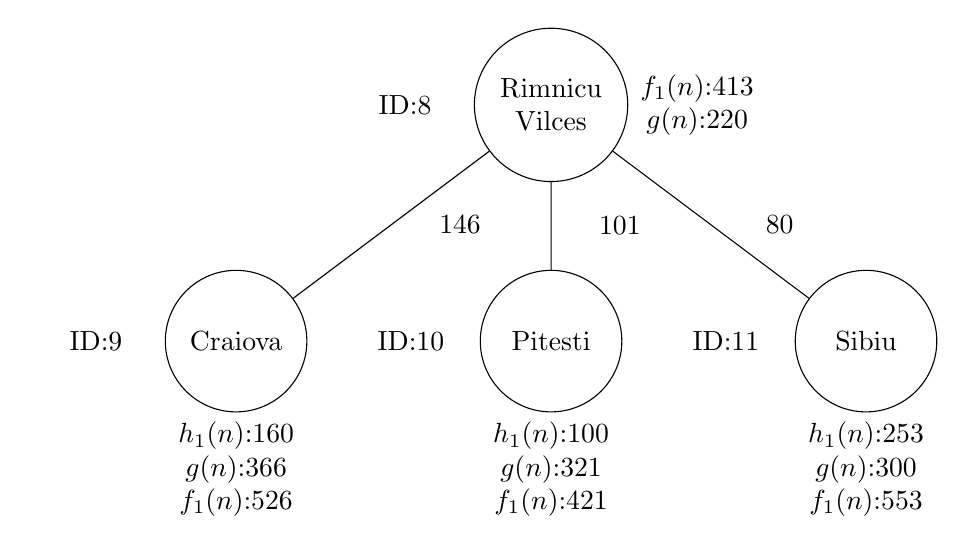
\begin{tikzpicture}[
    level 1/.style={sibling distance=40mm, level distance=30mm},
    every node/.style={text centered, text width=1.5cm},
    TreeNode/.style={circle, x radius = 3cm, y radius = 2cm, rotate=0, draw}
]

\node[TreeNode](a) {Rimnicu Vilces}
    child {
        node[TreeNode](b) {Craiova}
        edge from parent
            node[right] {146}
    }
    child {
        node[TreeNode](c) {Pitesti}
        edge from parent
            node[right] {101}
    }
    child {
        node[TreeNode](d) {Sibiu}
        edge from parent
            node[right] {80}
    };
    
\node also [label=right:$f_1(n)$:413\\$g(n)$:220] (a);
\node also [label=left:ID:8] (a);

\node also [label=left:ID:9] (b);
\node also [label=below:$h_1(n)$:160\\$g(n)$:366\\$f_1(n)$:526] (b);

\node also [label=left:ID:10] (c);
\node also [label=below:$h_1(n)$:100\\$g(n)$:321\\$f_1(n)$:421] (c);

\node also [label=left:ID:11] (d);
\node also [label=below:$h_1(n)$:253\\$g(n)$:300\\$f_1(n)$:553] (d);
%top:above, under:below
\end{tikzpicture}

\begin{thebibliography}{99}
\bibitem{citekey} %文献
\end{thebibliography}


\end{document}